%%%%%%%%%%%%%%%%%%%%%%%%%%%%%%%%%%%%%%%%%%%%%%%%%%%%%%%%%%%%%%%%%%%%%%%%%%%%%%%%%%%%%%%%%
%									TESIS DE DOCTORADO
%								CHRISTIAN FABIAN GARCIA ROMERO
%							   UNIVERSIDAD NACIONAL DE COLOMBIA
%
%%%%%%%%%%%%%%%%%%%%%%%%%%%%%%%%%%%%%%%%%%%%%%%%%%%%%%%%%%%%%%%%%%%%%%%%%%%%%%%%%%%%%%%%%


%%%%%%%%%%%%%%%%%%%%%%%%%%%%%%%%%%%%%%%%%%%%%%%%%%%%%%%%%%%%%%%%%%%%%%%%%%%%%%%%%%%%%%%%%

%SEGUNDO CAPITULO: ESTADO DEL CONOCIMIENTO

%%%%%%%%%%%%%%%%%%%%%%%%%%%%%%%%%%%%%%%%%%%%%%%%%%%%%%%%%%%%%%%%%%%%%%%%%%%%%%%%%%%%%%%%%

%----------------------------------------------------------------------------------------
% TITULO DEL CAPITULO 2
\chapter{Acoplamiento Flujo-Geomecánico}~\hypertarget{ch:chapter_02}{}
\label{ch:chapter_02}

\lipsum[1-2]

\bigskip

%----------------------------------------------------------------------------------------


%----------------------------------------------------------------------------------------
\section{Antecedentes Históricos}~\hypertarget{sec:sec210}{}
\label{sec:sec210}


%----------------------------------------------------------------------------------------


%----------------------------------------------------------------------------------------
\section{Metodologías de acoplamiento}~\hypertarget{sec:sec220}{}
\label{sec:sec220}

Un problema acoplado es aquel en que dos o más modelos físicos interactúan entre sí en busca de solucionar un problema y cuyo vinculo puede ocurrir en diferentes grados de interacción  \cite{Tran2005}. En un modelo hidro-geomecánico acoplado interactúan conjuntamente los modelos de flujo y geomecánico~\footnote{Se entiende como modelo \textit{geomecánico} el modelo de esfuerzos-deformación.}. Setarri \& Walters(2001) \cite{Settari2001} categorizaron diferentes tipos de acoplamiento que dependen del grado de interacción de los modelos físicos. Ese grado de interacción impacta en la exactitud de los resultados y en el costo computacional de las simulaciones. Pero esta clasificación se puede reducir a solo dos tipos de acoplamiento: (1) Modelos totalmente acoplados; (2) Modelos parcialmente acoplados.\bigskip

Los modelos totalmente acoplados combinan las ecuaciones que gobiernan los modelos de flujo y geomecánico en un solo sistema de ecuaciones. Las incógnitas que se resuelven en una simulación de flujo son las presiones de poros y las saturaciones de cada uno de los fluidos que conviven en el medio poroso. Las soluciones que se obtienen de una simulación geomecánica son los esfuerzos, deformaciones y desplazamientos. En un modelo totalmente acoplado se obtienen todas esas incógnitas de manera simultánea.\bigskip.

En los modelos parcialmente acoplados se realiza primero la simulación de un modelo físico ya sea flujo o geomecánico, obteniéndose los valores de las incógnitas. Esos valores entran al otro simulador como valores constantes y se obtienen los valores de las incógnitas de ese otro modelo físico. Luego se establece si el grado de convergencia es el deseado y de no serlo se continua con la siguiente iteración utilizando un método de convergencia como por ejemplo el de Newton-Raphson. Cuando la convergencia es la deseada se inicia el siguiente incremento de tiempo.\bigskip


%----------------------------------------------------------------------------------------


%----------------------------------------------------------------------------------------
\section{Modelamiento en Medios Porosos}~\hypertarget{sec:sec230}{}
\label{sec:sec230}

El modelamiento de problemas de geotecnia a menudo involucra problemas complejos relacionados con varias variables flujo-geomecánicas y los efectos de acoplamiento correspondientes. En comparación con muchos materiales de ingeniería, los suelos y las rocas exhiben un comportamiento esencialmente no-lineal y es normal que la solución analítica para tales problemas no exista.\bigskip

Es habitual en geotecnia, que los análisis de los problemas se hagan con información insuficiente sobre las condiciones iniciales “in situ”. Un ejemplo común es el caso de los proyectos de túneles o excavaciones en los que el diseño debe verificarse o complementarse utilizando información encontrada durante el desarrollo del proyecto. Por lo tanto, es importante que las simulaciones numéricas del problema se tomen como una herramienta rápida, confiable y poderosa para el análisis sistemático y para la toma de decisiones.\bigskip

La implementación de modelos numéricos y computacionales trae grandes beneficios, pero el uso ciego de estos modelos podría generar consecuencias negativas. Cuando se corre un modelo, siempre es tentador jugar con los parámetros que definen el problema y obtener buenos resultados, que en la mayoría de los casos no son realistas. Los modelos numéricos que procesan datos incorrectos, producirán resultados incorrectos. Aquí viene el importante papel del juicio del ingeniero. Este juicio debe abarcar todo el proceso, incluida la preparación de datos, el procesamiento del modelo y la verificación de resultados. Por lo tanto, es importante tener en cuenta que el modelamiento numérico es una tarea de ingeniería y no una función operativa de la computadora.\bigskip

En la actualidad existen programas comerciales basados en el método de los elementos finitos fáciles de usar y que permiten un modelamiento flujo-geomecánico muy efectivo. A pesar de esto, es difícil crear un modelo que permita un análisis realista de los procesos físicos involucrados en un proyecto real, debido a una serie de discrepancias entre la realidad y la predicción de los modelos numéricos.\bigskip

Cuando se usa uno de estos programas, el comportamiento mecánico del suelo se aproxima mediante un modelo constitutivo teórico que se formula en un marco de referencia continuo. La elección del modelo constitutivo y sus parámetros es una de las cuestiones más importantes a tener en cuenta al crear un modelo de elementos finitos para un proyecto geotécnico.\bigskip

El comportamiento constitutivo de un suelo o una roca, constituye la principal limitación en el proceso de modelamiento numérico. No importa que tan complejo sea nuestro modelo constitutivo, será siempre una simplificación del comportamiento real. Comúnmente el uso de software geotécnico donde se realizan un gran número de modelamientos numérico, se realiza sin comprender completamente los antecedentes y limitaciones de los modelos constitutivos y los métodos numéricos utilizados en el software.\bigskip

En proyectos reales resulta difícil validar el resultado de estas simulaciones, especialmente cuando estos no coinciden con lo que esperaría un ingeniero experto en el tema. Esto nos lleva a entender que es necesario establecer directrices sobre validación de modelamientos de elementos finitos en geotecnia. Esa fue la motivación principal para el Comité Geotécnico de NAFEMS para realizar una publicación sobre validación y verificación de modelos de elementos finitos para aplicaciones en geotecnia \cite{R.B.J.2013ValidationAnalysis}.\bigskip

NAFEMS es la “International Association for the Engineering Modelling, Analysis and Simulation Community”. El Comité Geotécnico de NAFEMS se creó en 2008 con el objetivo de desarrollar pautas para la aplicación práctica de métodos numéricos en geotecnia . En las siguientes tres secciones se resumirá las pautas establecidas por este grupo de trabajo para el modelamiento correcto en proyectos de geotecnia. Esas pautas se adaptaron para ser usados en simulaciones de problemas flujo-geomecánicos acoplados y se utilizaron como base metodológica para las predicciones hechas en este proyecto.


%........................................................................................
% TITULO DE LA SUBSECCIÓN 2.3.1
\subsection{Procesos en el Desarrollo de un Modelo}~\hypertarget{sec:sec231}{}
\label{sec:sec231}

En el momento que se pretende crear un modelo que represente lo mejor posible un fenómeno físico se debe dividir el proceso en la creación sistemática de varios tipos de modelos, desde un modelo más general hasta un modelo más específico. La lógica fluye del modelo conceptual, que es el más general, al matemático y el computacional que son más específicos. La \textbf{Figura} \ref{fig:fig21} muestra de manera muy simplificada el camino que hay que seguir para el desarrollo robusto de un modelo.\bigskip


El primer paso es comprender la compleja realidad del fenómeno físico y simplificarlo en un modelo conceptual. El principal objetivo de este paso es determinar los procesos cruciales de este fenómeno y reformular la realidad mediante la aplicación de simplificaciones, de tal forma que los fenómenos principales de esta realidad se conserven en el modelo conceptual. En la ~\MYhref[blue]{sec:sec32}{Sección 3.2} se detalla este tipo de modelo.\bigskip

El segundo paso es transformar este modelo conceptual en ecuaciones a través del modelo matemático. Este modelo se refiere a la formulación matemática de los procesos físicos identificados. Ejemplo de modelos matemáticos son el conjunto de Ecuaciones Diferenciales Parciales (EDP), que describen el equilibrio en un continuo. Otro ejemplo son los modelos constitutivos que describen el comportamiento mecánico de suelos y rocas. En la ~\MYhref[blue]{sec:sec33}{Sección 3.3} se detalla este tipo de modelos matemáticos.\bigskip

El tercer paso es transformar esas ecuaciones en un esquema numérico. Esto generalmente requiere una discretización del problema en el espacio y/o tiempo. Diferentes metodologías se pueden usar para esto. El uso de una u otra metodología depende en gran medida del fenómeno físico. Entre las más comunes en geomecánica están el Método de las Diferencias Finitas - (MDF), el Método de los Volúmenes Finitos - (MVF), el Método de los Elementos Discretos - (MED), el Método de los Elementos Finitos - (MEF), entre otros. En la ~\MYhref[blue]{sec:sec34}{Sección 3.4} se utiliza el MEF para la obtención del modelo numérico.\bigskip

%////////////////////////////////////////////////////////////////////////////////////////
% Figura 2.1
\begin{figure}[!ht]
\centering
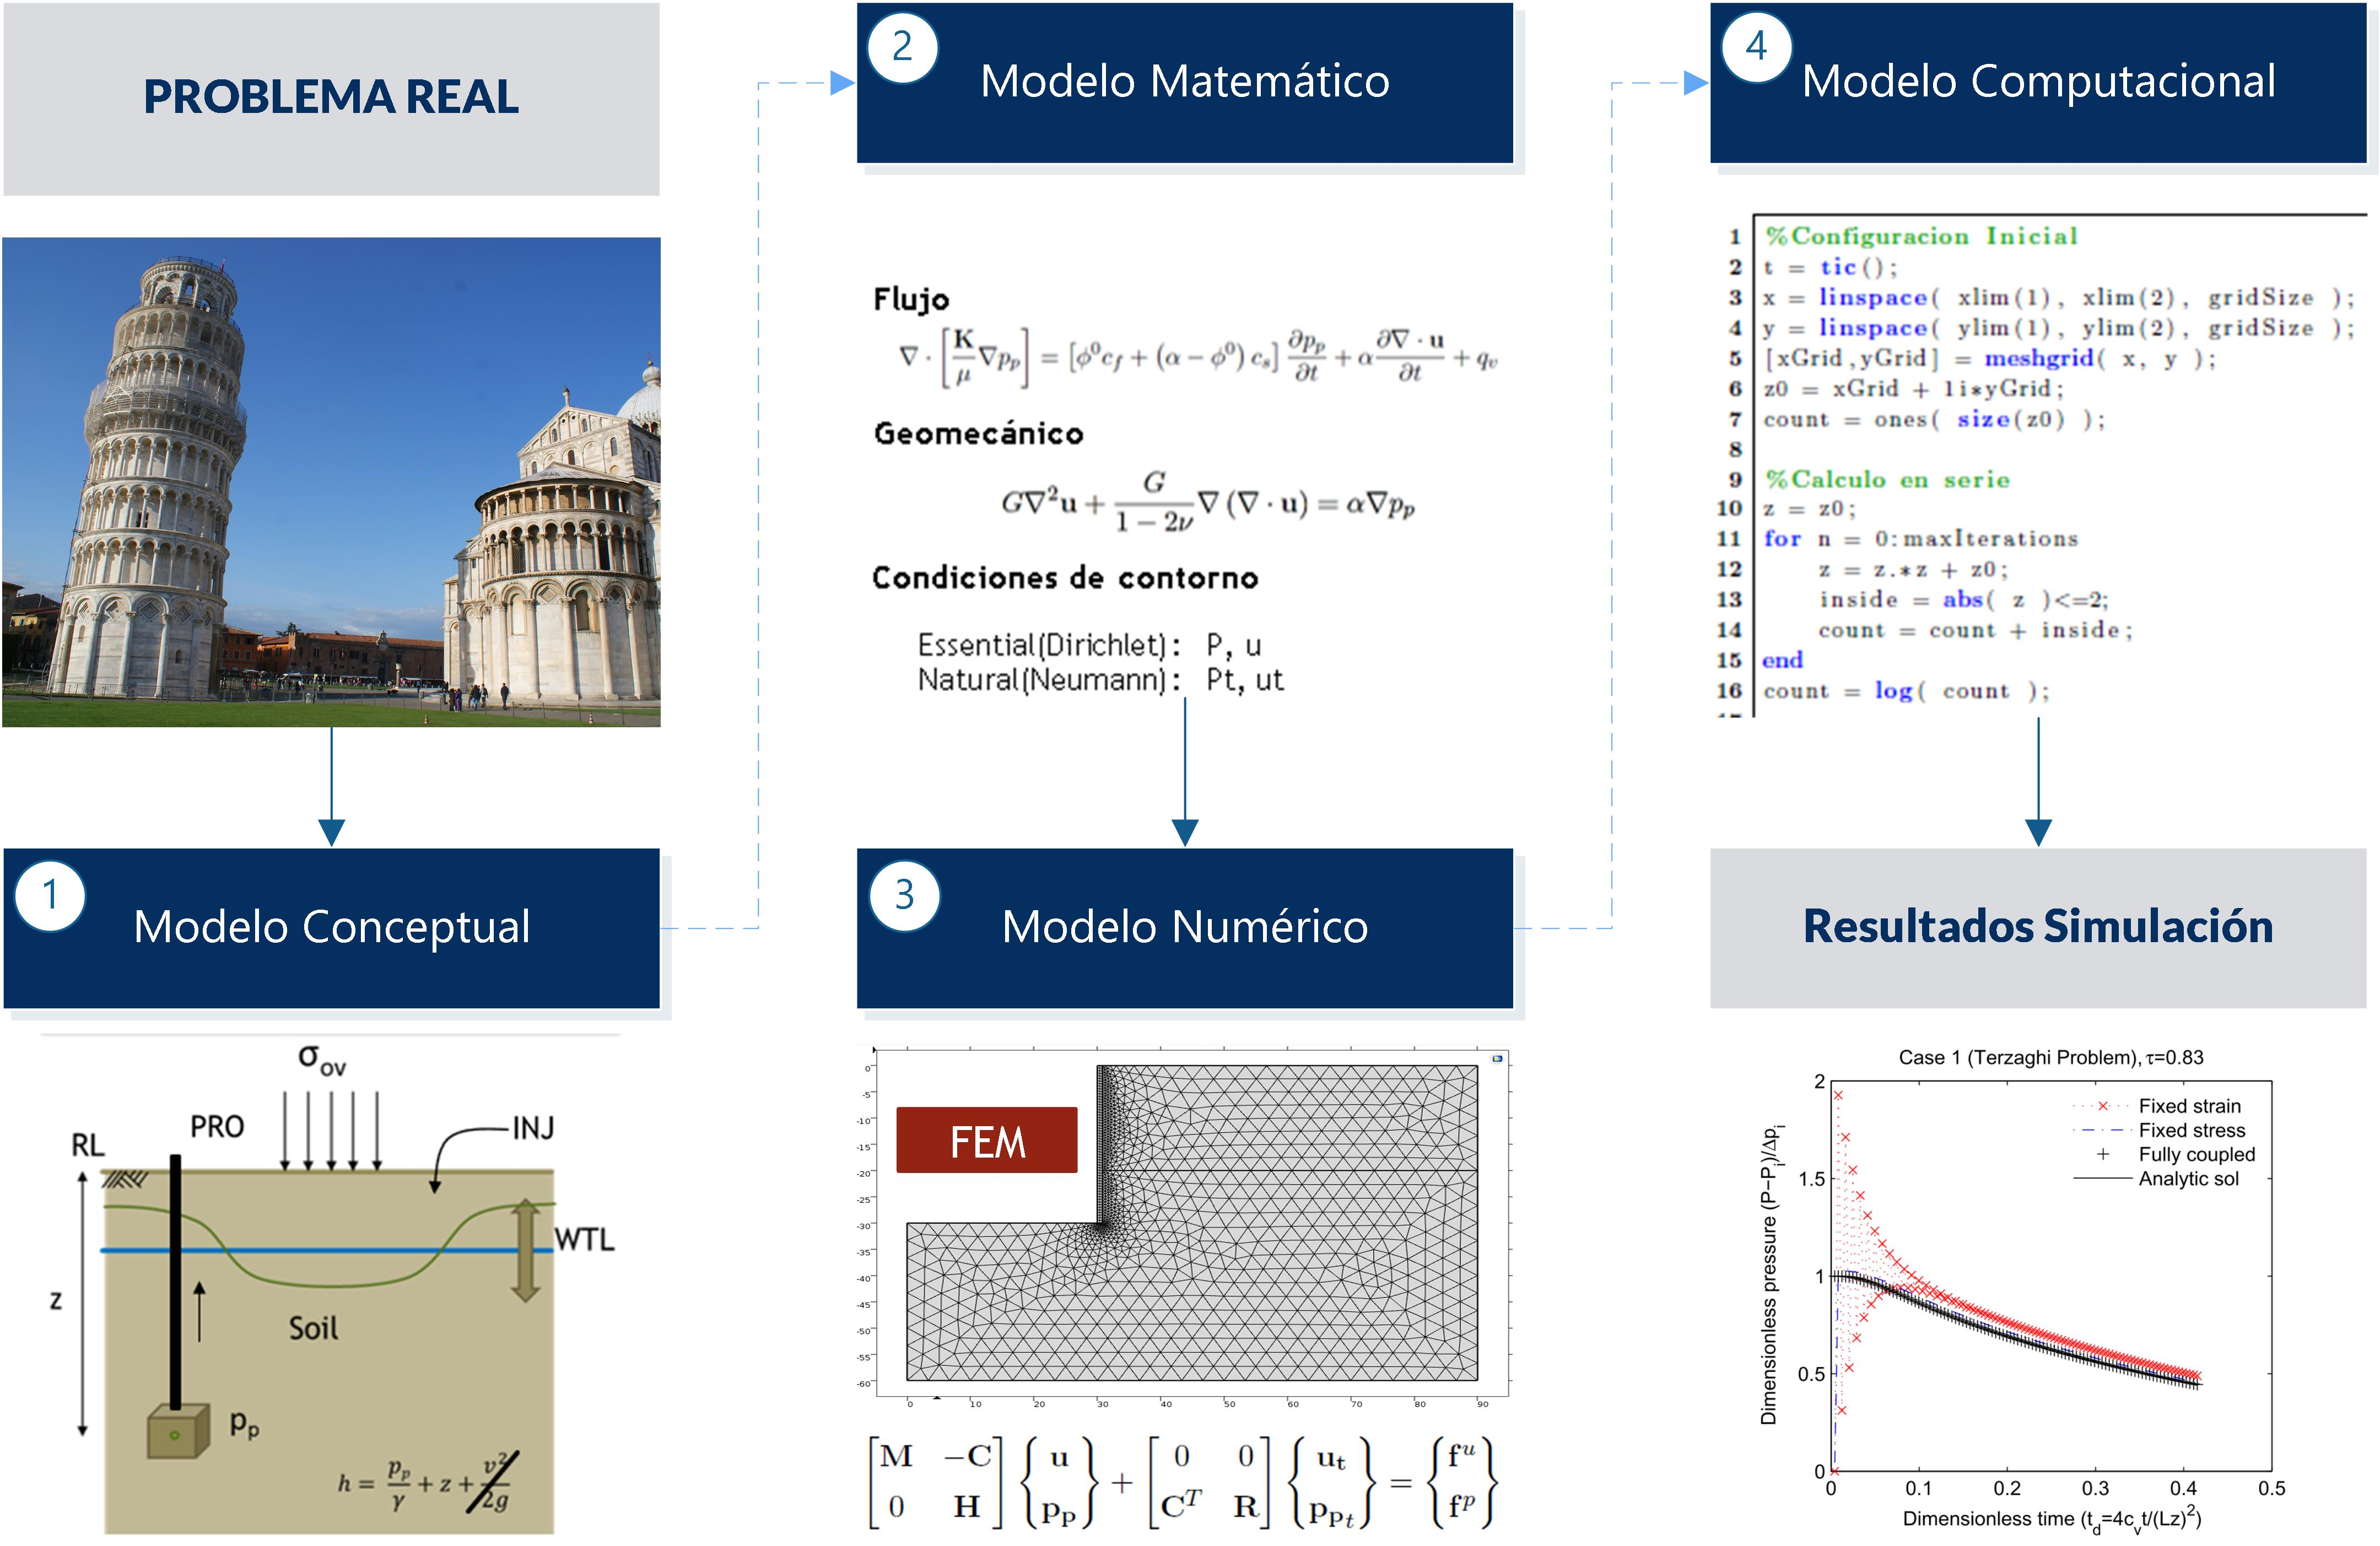
\includegraphics[width=16cm]{Imagenes/Kap_03/Desarrollo_de_Modelo.jpg}
\caption[Desarrollo de un modelo computacional]{Desarrollo de un modelo computacional. Modificado de Schwer(2006) \cite{Schwer2006GuideMechanics}}
\label{fig:fig21}
\end{figure}
%/////////////////////////////////////////////////////////////////////////////////////////


El último paso es la implementación del esquema numérico en un modelo computacional, usando un lenguaje de programación o usando un paquete de modelado. Los lenguajes más comunes usados en geomecánica son C/C++, Fortran y últimamente ha cogido mucho auge el uso de Python por su simplicidad y la curva de aprendizaje que es muy amable con los principiantes. Como paquetes de modelado se tiene Matlab y Abaqus, entre otros. Estos paquetes son muy comunes en ingeniería a pesar de no ser computacionalmente muy eficientes, son una alternativa viable para experimentación inicial, aunque un poco costosa. En este proyecto se usó Python para las simulaciones numéricas evidenciadas en la ~\MYhref[blue]{sec:sec35}{Sección 3.5}.\newpage

En softwares como Abaqus o Plaxis, común en proyectos geotécnicos, son los desarrolladores los que realizan la mayoría de los pasos anteriores y deciden sobre la formulación matemática, los esquemas numéricos y la implementación computacional. Por lo tanto, la responsabilidad de ellos es garantizar que estas simulaciones se acerquen los más posible a la realidad, cuando se les provee de datos de entrada fiables.\bigskip 

Para los usuarios de estos softwares, la división del proceso de modelado en diferentes pasos sigue siendo relevante, aunque su posición es diferente. Partiendo de un problema práctico de ingeniería, los usuarios crean varios modelos del problema y analizan los resultados para escoger el modelo que más se acerque a la realidad. Para escoger ese modelo deben realizar procesos de Verificación y Validación – (V\&V).\bigskip

Por lo tanto, el proceso más general para el desarrollo de un modelado en geomecánica debe incluir los pasos de V\&V. En la \textbf{Figura} \ref{fig:fig32} se observa el camino que hay que llevar para el desarrollo de un modelo geomecánico acoplado. En las secciones siguientes se explicará los pasos que conlleva la verificación y validación del modelo. En secciones posteriores se muestra las actividades desarrolladas para la creación de los modelos conceptual, matemático y numérico, aplicados en acoplamiento flujo-geomecánico. En el Capítulo 10 se muestran los resultados de las simulaciones numéricas hechas con el modelo computacional validado, en los casos de estudio propuestos en esta investigación.\bigskip

%////////////////////////////////////////////////////////////////////////////////////////
% Figura 2.2
\begin{figure}[!ht]
\centering
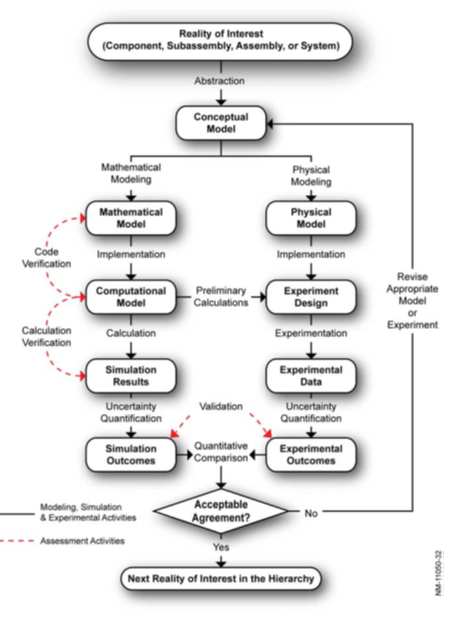
\includegraphics[width=11cm]{Imagenes/Kap_03/Desarrollo_modelo_geomecanico.png}
\caption[Proceso de desarrollo de un modelo geomecánico]{Proceso de desarrollo de un modelo geomecánico. Modificado de Schwer(2006) \cite{Schwer2006GuideMechanics}}
\label{fig:fig22}
\end{figure}
%/////////////////////////////////////////////////////////////////////////////////////////


%........................................................................................
% TITULO DE LA SUBSECCIÓN 2.3.2
\subsection{Verificación en Procesos de Modelamiento}~\hypertarget{sec:sec232}{}
\label{sec:sec232}

Existen varias definiciones para Verificación en procesos de modelamiento. NAFEMS en una de sus guías establece que \textit{“es el proceso de determinar que un modelo computacional representa con precisión el modelo matemático subyacente y su solución”} \cite{Schwer2006GuideMechanics}. Brinkgreve \& Engin (2013) \cite{R.B.J.2013ValidationAnalysis} definen Verificación como \textit{“el proceso de comprobación que un modelo o método ha sido implementado adecuadamente en un programa de computadora.”}\bigskip

Tomando en cuenta estas definiciones y lo que se muestra en la \textbf{Figura} \ref{fig:fig32}, la Verificación conlleva dos pasos: (1) Verificación de Código; (2) Verificación de Calculo. La verificación de código se establece a través de evidencia, de que tanto la formulación matemática y su correspondiente traducción a código están bien desarrollados. La verificación de cálculo se establece a través de evidencia, de que la solución discreta del modelo matemático es lo más precisa y exacta posible.\bigskip

% %////////////////////////////////////////////////////////////////////////////////////////
% % Figura 3.3
% \begin{figure}[!ht]
% \centering
% 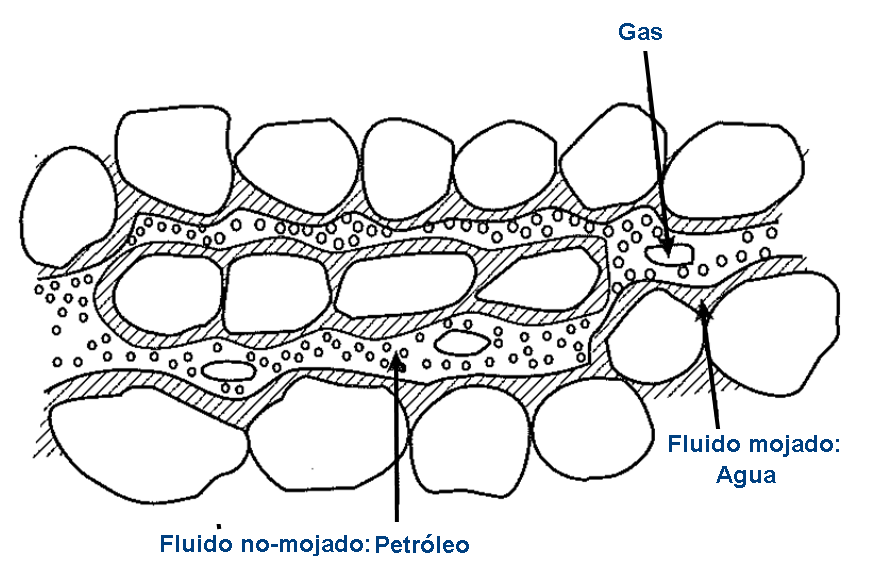
\includegraphics[width=7cm]{Imagenes/Mojabilidad.png}
% \caption[Proceso de verificación]{Proceso de verificación. Modificado de Schwer(2006) \cite{Schwer2006GuideMechanics}}
% \label{fig:fig33}
% \end{figure}
% %/////////////////////////////////////////////////////////////////////////////////////////

Entre las técnicas de verificación de código, el método más popular es comparar resultados de simulaciones con soluciones analíticas. Desafortunadamente pueden ocurrir dos situaciones al usar esta técnica. Que la solución analítica para determinado problema no exista, o que la solución analítica de dicho problema no sea de fácil implementación.\bigskip

Otra opción es usar softwares comerciales que hagan simulaciones del problema en cuestión. Luego se compara los resultados del software comercial con los resultados del código que se está verificando y se analizan los resultados. Esta técnica es viable siempre y cuando se tenga acceso a las licencias de esos paquetes de computador.\bigskip

Y una técnica que se puede usar con confianza es la llamada técnica de los \textit{Resultados Fabricados (“Manufactured Solutions”)}. El concepto básico de una solución fabricada es aparentemente simple. Dado una EDP y un código que proporciona soluciones generales de esa EDP, se fabrica una solución arbitraria, es decir inventada. \bigskip

Luego esa solución fabricada se substituye en la EDP junto con las condiciones de contorno e iniciales, también fabricadas. Como ya se tiene la solución del problema es solo comparar lo real con la predicción que realiza el modelo computacional propuesto y se hacen los análisis pertinentes.\newpage

En esta investigación se usaron las tres técnicas como verificación de los modelos matemático y computacional: (1) Para las simulaciones que se hacen en condiciones isotrópicas y elásticas se usó Abaqus para la verificación del código hecho en Python; (2) Para las simulaciones del modelo de flujo se usó MRST\footnote{Matlab Reservoir Simulation Toolbox (MRST). Ver (https://www.sintef.no/Projectweb/MRST/)}, que es un programa de código abierto hecho en Matlab para la simulación de modelos de flujo; (3) Para ciertas simulaciones iniciales, como la consolidación unidimensional y consolidación 2D, que se presentan al final de este capítulo, se usaron las soluciones analíticas existentes; (4) Para simulaciones de modelos constitutivos elastoplásticos del ~\MYhref[blue]{ch:chapter_5}{Capítulo 5}, se usaron “Soluciones Fabricadas” para la verificación de modelos de predicción constitutiva.\bigskip



%........................................................................................
% TITULO DE LA SUBSECCIÓN 2.3.3
\subsection{Validación en Procesos de Modelamiento}~\hypertarget{sec:sec233}{}
\label{sec:sec233}

Una definición propuesta por NAFEMS de Validación es “el proceso de determinar el grado en que un modelo es la representación exacta del mundo real desde la perspectiva de los usos previstos del modelo”. Otra definición es, “Validación es el proceso para hacer plausible que un modelo de computadora incluya las características esenciales para analizar una situación real y que los resultados obtenidos con el modelo sean representativos de esa realidad” \cite{R.B.J.2013ValidationAnalysis}.\bigskip

De una manera más simplificada la Validación tiene como objetivo evaluar la capacidad predictiva de un modelo. Esta evaluación se realiza comparando las predicciones realizadas por el modelo con los resultados de varias técnicas de Validación. Si estas comparaciones son satisfactorias, el modelo se considera validado para su propósito principal.\bigskip

Una de las razones para desarrollar un modelo, es realizar predicciones en los casos donde no se pudieran obtener datos experimentales. Pero según lo establecido en la \textbf{Figura} \ref{fig:fig32}, donde se ve el desarrollo de un modelo de predicción geomecánica, si se puede hacer la Validación de los resultados entre las simulaciones numéricas y experiencias de laboratorio, este modelo queda validado para ser usado en aplicaciones reales.\bigskip

En pocas palabras, si el modelo pasa las pruebas de validación propuestas con el uso de experiencias de laboratorio, luego puede usarse para hacer las predicciones deseadas con confianza, para el uso previsto. Cuando se dice que el modelo está validado para el uso previsto, no es solo el modelo computacional, sino los modelos matemático y conceptual los que quedan validados. Es a través de la validación del modelo conceptual que se gana confianza, de que la física del problema se incluyó de manera correcta en el desarrollo del modelo. Las distintas técnicas de validación que se pueden usar son:\bigskip

\begin{itemize}
    \item Comparación con medidas de campo cuando el proyecto está en construcción
    \item Comparación con software comerciales
    \item Comparación con resultados de pruebas de laboratorio
    \item Comparación con \textit{Benchmarks}
\end{itemize}

En este proyecto se utilizaron tres de las cuatro técnicas expuestas: Comparaciones con simulaciones de Abaqus, resultados de pruebas de laboratorio (i.e. Triaxial, edométrica, compresión inconfinada.) y uso de \textit{Benchmarks}.\bigskip

Un \textit{Benchmarks}, en el marco de V\&V, es un problema de ejemplo bien definido para el cual existe una solución de referencia. El término \textit{Benchmarking} se puede definir como el proceso para evaluar la variación en los resultados de diferentes modelos para un problema de ejemplo bien definido. La solución de un \textit{Benchmarks} no es una solución exacta, pero es una solución de referencia que se considera estándar para ese problema en particular.\bigskip

La mayoría de \textit{Benchmarks} son problemas prácticos simplificados para los cuales no existe una solución analítica. Una serie de \textit{Benchmarks} para geotecnia han sido definida y publicados en Jeffries (1995); Schweiger (1998, 2002, 2006); Andersen et al. (2005).\bigskip



%........................................................................................
% TITULO DE LA SUBSECCIÓN 2.3.4
\subsection{Discrepancias en Procesos de Modelamiento}~\hypertarget{sec:sec234}{}
\label{sec:sec234}

La identificación de posibles discrepancias puede resultar en una mejora del modelo y una
posible reducción del error en general. También puede permitir una cuantificación de las incertidumbres de los parámetros de diseño y su posible rango de valores. Según Brinkgreve \& Engin (2013) \cite{R.B.J.2013ValidationAnalysis}, las discrepancias se pueden dividir en las siguientes categorías: (1) Simplificaciones; (2) Errores de modelamiento; (3) Modelos constitutivos; (4) Incertidumbres.

%----------------------------------------------------------------------------------------
\subsubsection{Simplificaciones}~\hypertarget{sec:sec2341}{}
\label{sec:sec2341}

Las simplificaciones son el resultado de las elecciones realizadas por el modelador. Estas simplificaciones son hechas en diferentes partes del proceso de modelamiento, pero en su mayoría son hechas en el modelo conceptual. Ejemplos de simplificaciones son:

\begin{itemize}
    \item Simplificaciones de geometría del dominio del problema
    \item Selección del alcance del modelo
    \item Simplificaciones en el comportamiento mecánico de rocas y suelos
    \item Simplificaciones en el proceso de construcción
\end{itemize}


%----------------------------------------------------------------------------------------
\subsubsection{Errores de Modelamiento}~\hypertarget{sec:sec2342}{}
\label{sec:sec2342}

Durante el proceso de modelamiento en acoplamiento geomecánico. El proceso de validación puede ayudar a identificar y cuantificar tales errores de modelamiento. Se pueden generar errores debido a:

\begin{itemize}
    \item Errores en los datos de entrada
    \item Errores de discretización o mallado
    \item Adopción de condiciones de contorno e iniciales erradas
    \item Integración en el tiempo no adecuada
    \item Adopción de teorías y métodos no representativos del problema
\end{itemize}

%----------------------------------------------------------------------------------------
\subsubsection{Modelos Constitutivos}~\hypertarget{sec:sec2343}{}
\label{sec:sec2343}

Probablemente la parte más importante del modelamiento numérico en acoplamiento geomecánico es la selección correcta del modelo constitutivo del medio y sus parámetros. El comportamiento mecánico de suelos y rocas reales está influenciado por una buena cantidad de parámetros que pueden ser medidos en laboratorio y/o \textit{“in situ”}, pero que son muy difíciles de incluir en una formulación matemática robusta. Aquí se destacan diferentes aspectos del modelado constitutivo que generan discrepancias:

\begin{itemize}
    \item No unicidad relacionada con la plasticidad
    \item Comportamiento no-drenado
    \item Comportamiento no-saturado
    \item Trayectorias de esfuerzo no representativas del problema
\end{itemize}

%----------------------------------------------------------------------------------------
\subsubsection{incertezas}~\hypertarget{sec:sec2344}{}
\label{sec:sec2344}

En un proyecto real hay muchos aspectos que no son conocidos o no se pueden medir con exactitud. Por lo tanto, existen una seria de incertezas que influyen en el modelamiento y generan errores. Ejemplos de incertezas son:

\begin{itemize}
    \item Datos de los suelos o rocas imprecisos o inexistentes
    \item Variación espacial de las propiedades del suelo o roca
    \item Diseño \textit{versus} construcción real
\end{itemize}



%----------------------------------------------------------------------------------------

%----------------------------------------------------------------------------------------
\section{Retos en Acoplamiento Geomecánico}~\hypertarget{sec:sec240}{}
\label{sec:sec240}




%----------------------------------------------------------------------------------------


%----------------------------------------------------------------------------------------
% \section{Conclusiones del estado del conocimiento}~\hypertarget{sec:sec240}{}
% \label{sec:sec240}


\bigskip
%----------------------------------------------------------------------------------------
